\documentclass[10pt,twocolumn,letterpaper]{article}
\usepackage[dvipsnames]{xcolor}
\usepackage[pagebackref,breaklinks,colorlinks,citecolor=cvprblue]{hyperref}
\usepackage{amsmath}
\usepackage{amssymb}
\usepackage{tikz}
\usepackage{pgfplots}
\pgfplotsset{compat=1.17}
\usetikzlibrary{pgfplots.groupplots}
\usepackage[pagebackref,breaklinks,colorlinks]{hyperref}
\def\addlegendimage{\pgfplots@addlegendimage}

\begin{document}

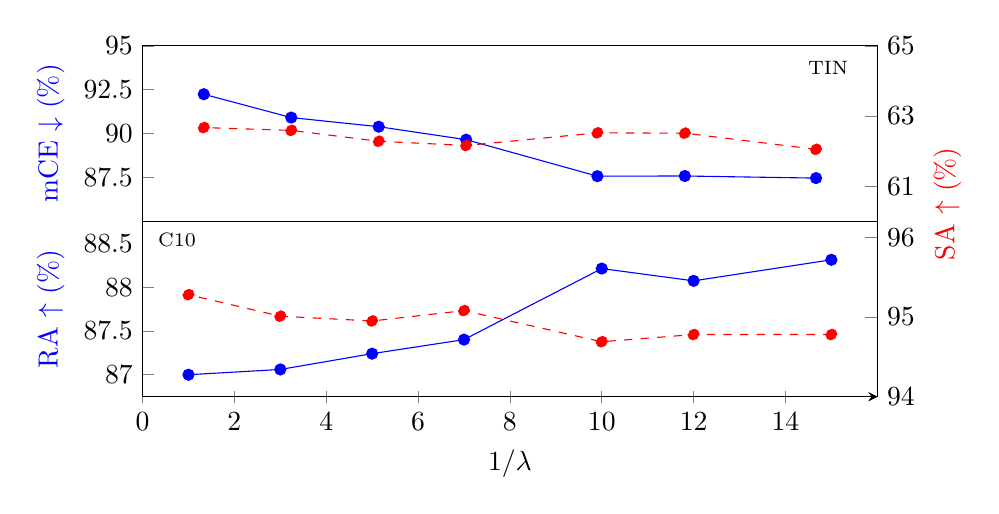
\begin{tikzpicture}        
\begin{groupplot}[
    group style={
        group name=my fancy plots,
        group size=1 by 2,
        xticklabels at=edge bottom,
        vertical sep=0pt
    },
    width=0.9\linewidth,
]

\nextgroupplot[ymin=85,ymax=95,
               ytick={87.5, 90, ..., 95},
               xtick=\empty,
               ytick pos=left,
               % axis x line=top, 
               % axis y discontinuity=parallel,
               height=1.5in,
               ylabel={\color{blue}{mCE} $\downarrow$ (\%)},
               legend image post style={scale=0},
               legend style={draw=none}
]
\addplot[mark=none] coordinates {(0, 0)};
\addlegendentry{\scriptsize TIN};
\addplot[mark=*,blue] coordinates {
      (15, 87.46)
      (12, 87.58)
      (10, 87.57)
      (7, 89.65)
      (5, 90.39)
      (3, 90.91)
      (1, 92.24)
    };

\nextgroupplot[ymin=86.75,ymax=88.75,
               axis x line=bottom,
               ytick={87, 87.5, 88, 88.5},
               xtick pos=lower,
               ytick pos=left,
               height=1.5in,
               xlabel={$1 / \lambda$},
               xmin=0,
               xmax=16,
               xtick={0, 2, 4, ..., 15},
               ylabel={\color{blue}{RA} $\uparrow$ (\%)},
               legend image post style={scale=0},
               legend style={draw=none},
               legend style={at={(0,1)},anchor=north west}
]
\addplot[mark=none] coordinates {(0, 0)};
\addlegendentry{\scriptsize C10};

\addplot[mark=*,blue] coordinates {
      (15, 88.31)
      (12, 88.07)
      (10, 88.21)
      (7, 87.40)
      (5, 87.24)
      (3, 87.06)
      (1, 87.00)
    };

\end{groupplot}

\begin{groupplot}[
    group style={
        group name=my fancy plots,
        group size=1 by 2,
        vertical sep=0pt,
    },
    width=0.9\linewidth,
]

\nextgroupplot[ymin=60,ymax=65,
               ytick={61, 63, ..., 65},
               xtick=\empty,
               ytick pos=right,
               % axis x line=top, 
               % axis y discontinuity=parallel,
               height=1.5in
               ]
\addplot[mark=*,red,dashed] coordinates {
      (15, 62.05)
      (12, 62.51)
      (10, 62.52)
      (7, 62.16)
      (5, 62.28)
      (3, 62.59)
      (1, 62.67)
    };

\nextgroupplot[ymin=94,ymax=96.2,
               axis x line=bottom,
               ytick={94, 95, ..., 96},
               xtick=\empty,
               ytick pos=right,
               height=1.5in,
               xmin=0,
               xmax=16,
               ylabel={\color{red}{SA} $\uparrow$ (\%)},
               every axis y label/.append style={at=(ticklabel cs:1.1)}
]
\addplot[mark=*,red,dashed] coordinates {
      (15, 94.78)
      (12, 94.78)
      (10, 94.69)
      (7, 95.08)
      (5, 94.95)
      (3, 95.01)
      (1, 95.28)
    };
\end{groupplot}
\end{tikzpicture}

\end{document}